% --------------------------------------------------------------------------
% Template for IWAENC 2022 papers; to be used with:
%          spconfa4.sty  - ICASSP/ICIP LaTeX style file, and
%          IEEEbib.bst - IEEE bibliography style file.
%
% (Last modified by H. Loellmann, LMS, FAU Erlangen-Nuremberg, Jan. 2020)
%
% --------------------------------------------------------------------------

\documentclass{article}
\usepackage[preprint]{spconfa4}
\usepackage{amsmath,graphicx}
\usepackage[dvipsnames]{xcolor}
\usepackage{tikz}
\usetikzlibrary{arrows,snakes,backgrounds,matrix,patterns,positioning,fadings}
\usepackage{standalone}
\usepackage{subfig}
\usepackage{upgreek}
\usepackage{nicefrac}
\usepackage{dsfont}
\usepackage{bm}
\usepackage{cancel}
\usepackage{amsbsy}
\usepackage{algorithm}
\usepackage{algpseudocode}
\usepackage{lipsum}
\usepackage{harpoon}
\usepackage{comment}
\newenvironment{note}
 {\par\textcolor{Blue}{\bfseries Note:} \color{Blue}\ignorespaces}
 {\par}
\newenvironment{attention}
 {\par\textcolor{red}{\bfseries Attention:} \color{red}\ignorespaces}
 {\par}
\usepackage{hyperref}
\hypersetup{
	colorlinks,
	linkcolor={blue!80!black},
	citecolor={blue!80!black},
	urlcolor={blue!80!black}
}

\newcommand{\mtxb}[1]{\bm{\mathrm{#1}}}
\newcommand{\T}{{\mathrm{T}}}
\newcommand{\herm}{{\mathrm{H}}}
\newcommand{\ev}[1]{\mathrm{E} \left\lbrace #1 \right\rbrace}

% \excludecomment{note}
% \excludecomment{attention}

% Common variables
\newcommand{\h}{\mtxb{h}}
\newcommand{\x}{\mtxb{x}}
\newcommand{\R}{\mtxb{R}}
\newcommand{\w}{\mtxb{w}}
\newcommand{\z}{\mtxb{z}}
\newcommand{\uu}{\mtxb{u}}
\newcommand{\aRho}{\mtxb{P}}
\newcommand{\hf}{{\bm{h}}}
\newcommand{\xf}{{\bm{x}}}
\newcommand{\Rf}{{\bm{{R}}}}
\newcommand{\wf}{{\bm{w}}}
\newcommand{\zf}{{\bm{z}}}
\newcommand{\uuf}{{\bm{u}}}
\newcommand{\aRhof}{{\bm{{P}}}}
\newcommand{\I}{\mtxb{I}}
\newcommand{\Cset}{\mathcal{C}}
\newcommand{\Csetb}{\bar{\mathcal{C}}}
\newcommand{\Mset}{\mathcal{M}}
\newcommand{\Nset}{\mathcal{N}}



% IMPORTANT: Add copyright notice by uncommenting the appropriate line
%----------------------------------------------------------
% For papers in which all authors are employed by the US government,
% \copyrightnotice{U.S. Government work not protected by U.S. copyright}

% For papers in which all authors are employed by a Crown government (UK, Canada, and Australia)
% \copyrightnotice{978-1-6654-6867-1/22/\$31.00~\copyright2022 Crown}

% For papers in which all authors are employed by the European Union,
% \copyrightnotice{978-1-6654-6867-1/22/\$31.00~\copyright2022 European Union}

% For all other papers the copyright notice is
\copyrightnotice{978-1-6654-6867-1/22/\$31.00~\copyright2022 IEEE}

% Title.
% ------
\title{CROSS-RELATION-BASED FREQUENCY-DOMAIN\\ BLIND SYSTEM IDENTIFICATION USING ONLINE ADMM}
%
% Single address.
% ---------------
\name{Matthias Blochberger\sthanks{This research work was carried out at the ESAT Laboratory of KU Leuven, in the frame of the SOUNDS European Training Network. This project has received funding from the European Union's Horizon 2020 research and innovation programme under the Marie Skłodowska-Curie grant agreement No. 956369.}, Filip Elvander\sthanks{This work was supported in part by the Research Foundation - Flanders (FWO) grant 12ZD622N.}, ... who else?}
\address{KU Leuven\\Department of Electrical Engineering (ESAT)\\STADIUS Center for Dynamical Systems, Signal Processing and Data Analytics \\3001 Leuven, Belgium}
%
\begin{document}
%\ninept
%
\maketitle
%
\begin{abstract}
    In this contribution, we propose a cross-relation-based adaptive algorithm for blind identification of single-input multiple-output (SIMO) systems in the frequency domain using the alternating direction method of multipliers (ADMM).
    The proposed algorithm exploits the separability of the cross-channel relations by splitting the multichannel identification problem into lower-dimensional sub-problems with lowered computational complexity, which can be solved in parallel.
    Each sub-problem yields estimates for a subset of channel frequency responses, which then are combined into a consensus estimate per channel using general form consensus ADMM in an adaptive updating scheme.
    With numerical simulations, we show that it is possible to achieve convergence speeds comparable to low-cost frequency-domain algorithms and estimation errors better than a high-performing Quasi-Newton method.
\end{abstract}
%
\begin{keywords}
    blind system identification, multichannel signal processing, ADMM, Online-ADMM
\end{keywords}
%
\section{Introduction}
\label{sec:intro}


The problem of blind system identification (BSI), which aims to estimate channel impulse responses of an unknown system without knowing the input signal, has been subject of extensive research over the recent decades.
First introduced in \cite{satoMethodSelfRecoveringEqualization1975}, various methods have been proposed since.
Early methods use higher-order statistics \cite{godardSelfRecoveringEqualizationCarrier1980,tongNewApproachBlind1991,mecidel1991tutorial} for channel estimation, however high complexity led to research into methods only using second-order statistics.
One of the first to be proposed was the cross-relation (CR) method \cite{tong1994blind, guanghanxuLeastsquaresApproachBlind1995}, with other relevant approaches being subspace methods \cite{moulinesSubspaceMethodsBlind1995,gannotSubspaceMethodsMultimicrophone2003,diamantarasEfficientSubspaceMethod2008,mayyalaStructureBasedSubspaceMethod2017} and maximum-likelihood \cite{yingbohuaFastMaximumLikelihood1996} methods.

\noindent Out of various multichannel BSI algorithms which have been proposed, adaptive cross-relation-based least mean squares (LMS) algorithms in time and frequency domain \cite{huangAdaptiveMultichannelLeast2002,huangClassFrequencydomainAdaptive2003} are the ones most widely used.
The NMCFLMS algorithm is an efficient algorithm utilizing the fast Fourier transform (FFT) which has been extended to include constraints to improve robustness to noise and performance on acoustic impulse responses (RNMCFLMS \cite{huNoiseRobustBlind2015}, \(l_p\)-RNMCFLMS \cite{heNoiseRobustFrequencyDomain2018}, phase-constrained-\(l_p\)-RNMCFLMS \cite{joRobustBlindMultichannel2021}).
Further, the quasi-Netwon \cite{habetsOnlineQuasiNewtonAlgorithm2010} approach in the time domain utilizes a BFGS method to estimate the Hessian of the problem.

The alternating direction method of multipliers (ADMM) \cite{boydDistributedOptimizationStatistical2011} solves convex optimization problems by splitting them into smaller sub-problems, each less complex to solve than the original one.
It has found applications in a large number of areas such as machine learning or control systems.
Here, we use ADMM to separate the inter-channel cross-relations to form smaller sub-problems involving overlapping subsets of the entire channel set and use equality constraints to find a consensus on the overlapping estimated sub-problem parameters.
The ADMM update steps are applied in a block processing scheme forming an adaptive algorithm also referred to as Online-ADMM \cite{wangOnlineAlternatingDirection2013,hosseiniOnlineDistributedADMM2014}.

The resulting algorithm provides good estimation results while keeping complexity low and providing scalability through parallel processing possibilities.


% \lipsum[1-4]

% #############################################################################
% #############################################################################
\section{Problem statement}
\label{sec:problem_statement}


% #############################################################################
\subsection{Signal Model}
\label{ssec:signal_model}
We consider an acoustic SIMO system with the input signal \(\mtxb{s}(n)\) and \(i \in \Mset\) with \(\Mset \triangleq \{1,\ldots,M\} \) outputs \(\x_i(n)\) defined as
\begin{align}
    \mtxb{s}(n) &= \begin{bmatrix}
        s(n)&s(k-1)&\ldots&s(k-2L+2)
    \end{bmatrix}^{\T},\\
    \x_i(n) &= \begin{bmatrix}
        x_i(n)&x_i(k-1)&\ldots&x_i(k-L+1)
    \end{bmatrix}^{\T}.
\end{align}
Each output \(\x_i(n)\) is the convolution of \(\mtxb{s}(n)\) with the respective channel impulse response \(\h_i\) and an additive noise term \(\mtxb{v}_i(n)\), assumed to be zero-mean and uncorrelated.
The signal model is described by
\begin{equation}
    \x_i(n) = \mtxb{H}_i \mtxb{s}(n) + \mtxb{v}_i(n),
\end{equation}
where \(\mtxb{H}_i\) is the \(L \times (2L-1)\) linear convolution matrix of the \(i\)th channel using the elements of \(\h_i\).

% #############################################################################
\subsection{Cross-relation approach}
\label{ssec:cross_rel}
The cross-relation approach for BSI aims to use output signals of the system only to identify it.
This can be achieved by exploiting the relative channel information when more than one channels are available, and the identifiability conditions \cite{guanghanxuLeastsquaresApproachBlind1995} are satisfied. These conditions are: (i) the channel transfer functions have no common zeros (i.e. are not co-prime), and (ii) the covariance matrix of the input signal \(\mtxb{s}(n)\) is of full rank (i.e. the signal fully excites the channels).

The fundamental equality of this approach, here in the noiseless case \(\mtxb{v}_i(n) = 0\), is 
\begin{equation}
    \x_i^{\T}(n) \h_j = \x_j^{\T}(n) \h_i,\quad i,j \in \Mset,\,i\neq j\label{eq:cross_rel:equality_conv}
\end{equation}
which states that the channel output signal convolved with the impulse response of another is equal to the vice-versa as follows from the commutativity property of the convolution.
Left-multiplication and applying the expectation operator to form the covariance matrix \(\R_{ij} = \ev{\x_i \x_j^\T}\) and combining all cross-relations \eqref{eq:cross_rel:equality_conv} (see e.g. \cite{huangAdaptiveMultichannelLeast2002} for a more thourough derivation) yields the system of equations  
\begin{equation}
    \R(n) \h = \bm{0}, \label{eq:cross_rel:null_space}\\
\end{equation}
where 
\begin{equation}
    \R = \begin{bmatrix}
        \sum_{m \neq 1} \R_{mm} & -\R_{21} & \cdots & -\R_{M1}\\
        -\R_{12} & \sum_{m \neq 2} \R_{mm} & \cdots & -\R_{M2}\\
        \vdots & \vdots & \ddots & \vdots\\
        -\R_{1M} & -\R_{2M} & \cdots & \sum_{m \neq M} \R_{mm}\\
    \end{bmatrix},\label{eq:cross_rel:data_matrix}
\end{equation}
and \(\h = \begin{bmatrix}
    \h_1^\T & \cdots & \h_M^\T
\end{bmatrix}^\T\).
Looking at the problem in the frequency domain, the derivation is analogous. We denote all frequency-domain variables in bold cursive (e.g. \(\Rf\)) compared to the time-domain bold upright (e.g \(\R\)). The derivation involves the frame-based overlap-save technique, working with signal frames \(\x_{i,2L}(m)\) with length \(2L\), frame index \(m\), leading to the system of equations 
\begin{equation}
    \Rf(m) \hf = \bm{0} \label{eq:frequency_domain:null_space}\\
\end{equation}
where the matrix is recursivly computed by \begin{equation}
    \Rf(m) = \eta \Rf(m-1) + (1-\eta )\hat{\Rf}(m)
\end{equation}
instead of estimating the expectation by sample averages. Here, \(\eta \in [0,1]\) is an exponential smoothing factor and \(\hat{\Rf}(m)\) is constructed analogous to \eqref{eq:cross_rel:data_matrix}, however with covariance matrices replaced by cross-spectrum matrices 
\begin{equation}
    \Rf_{ij}(m) = \bm{{S}}_{i}^\herm (m) \bm{{S}}_{j}(m),
\end{equation}
with 
\begin{equation}
    \bm{{S}}_{i}(m) = \bm{{W}}^{01}_{L \times 2L} \bm{{D}}_{i}(m) \bm{{W}}^{10}_{2L \times L}.
\end{equation}
The matrix \(\bm{{D}}_{i}(m) = \operatorname{diag} \left\{ \operatorname{FFT}_{2L} \left\{ \x_{i,2L}(m) \right\} \right\}\) contains the  signal spectrum on its diagonal and the overlap-save matrices are defined as
\begin{align}
    \mtxb{W}_{L \times 2L}^{01} &= \begin{bmatrix}
        \mtxb{0}_{L \times L} & \mtxb{I}_{L \times L}
    \end{bmatrix},\\
    \mtxb{W}_{2L \times L}^{10} &= \begin{bmatrix}
        \mtxb{I}_{L \times L} & \mtxb{0}_{L \times L}
    \end{bmatrix}^\T,\\
    \bm{{W}}_{2L \times L}^{01} &= \mtxb{F}_{L \times L} \mtxb{W}_{L \times 2L}^{01} \mtxb{F}_{2L \times 2L}^{-1},\\
    \bm{{W}}_{2L \times L}^{10} &= \mtxb{F}_{2L \times 2L} \mtxb{W}_{2L \times L}^{10} \mtxb{F}_{L \times L}^{-1},
\end{align} where $\mtxb{F}$ is the DFT matrix for sizes L and 2L.
Analogous to the time-domain formulation, the vector \(\hf\) is a stacked vector of complex-valued frequency responses.
In the presence of noise, the system of equations \eqref{eq:frequency_domain:null_space} is best solved by posing it as a least-mean-squares minimization problem.
%  minimizing \(\|\underline{\bm{e}} \|^2 = \| \Rf \hf \|^2\) with the constraint \(\hf^\herm \hf = a\) to avoid the trivial zero solution.
% As this effectively seeks the \(a\)-scaled eigenvector of the squared hermitian matrix \(\Rf^\herm \Rf\) corresponding to the smallest eigenvalue, we can replace it with its non-squared form \(\Rf\) as the eigenvectors for both are equal.
To compute the estimates, we minimize the cost function
\begin{equation}
    J(\hf)(m+1) = \hf^\herm(m) \Rf(m) \hf(m),\label{eq:frequency_domain:cost_function}
\end{equation}
as the minimization problem
\begin{align}
    \hat{\hf}(m+1) = \arg \min_{\hf} \quad &\hf^\herm(m) \Rf(m) \hf(m), \label{eq:frequency_domain:min_prob}\\
    \text{s.t. } \quad &\hf^\herm(m) \hf(m) = a.
\end{align}
In the following section, we introduce a novel adaptive method to find a solution to this problem.

% #############################################################################
% #############################################################################
\section{Proposed Method}
\label{sec:proposed_method}

% #############################################################################
\subsection{Problem Splitting}
\label{ssec:problem_splitting}
In state-of-the-art algorithms \cite{heNoiseRobustFrequencyDomain2018,habetsOnlineQuasiNewtonAlgorithm2010}, the minimization problem \eqref{eq:frequency_domain:min_prob} is solved in its full form resulting in potentially high computational effort when the number of channels and length of impulse responses or number of DFT bins is large.
Here however, we split the problem into \(N \in \mathbb{N}\) sub-problems and denote the index set of these \(N\) sub-problems as \(\Nset \triangleq \{1,\ldots,N\}\).
Each sub-problem is defined by a subset of the full channel set \(\Cset_i \subseteq \Mset\) with \(i \in \Nset\).
Following from that, we define the sets \(\Csetb_j = \left\{ i \vert j \in \Cset_i \right\}\) for \(i,j \in \Mset\) which is the set of sub-problems a channel  \(j\) is part of.
This channel-to-sub-problem relation can also be expressed as a \(M \times P\) matrix \(\mtxb{G}\) where the sets \(\Cset_i\) and \(\Csetb_j\) are the indices of non-zero elements of the rows and columns respectively (see \autoref{fig:problem_splitting:problem_splitting_matrix}).
Further, \(M_i = \left| \Cset_i \right| \) and \(N_j = \left| \Csetb_j \right| \) with \(i,j \in \Mset\). 
We replace the cost function \eqref{eq:frequency_domain:cost_function} with the separable cost function 
\begin{equation}
    \tilde{J}(\hf) = \sum_{i \in \Nset} \tilde{J}_i(\wf_i)  = \sum_{i \in \Nset} \wf_i^\T \aRhof_i \wf_i
    \label{eq:problem_splitting:cost_function}
\end{equation}
where \(\wf_i\) is defined as the stacked vector of estimated frequency responses analogous to \(\hf\) (cf. \autoref{ssec:cross_rel}) and \(\aRhof\) is constructed as defined in \eqref{eq:cross_rel:data_matrix}, both using the respective subset \(\Cset_i\).
If the channel subsets are proper \(\Cset_i \subset \Mset\), this leads to \(N\) sub-problems each with smaller dimensions than the original centralized problem, reducing complexity.
The lowest-dimensionality is attained when each \(\Cset_i\) has two elements, i.e. two channels, with parallel processing, effectively reducing problem size from \(ML \times ML\) to \(2L \times 2L\).
In \autoref{fig:problem_splitting:problem_splitting_matrix}, we try to visualize which information is used to solve the sub-problems in relation to the initial problem for a general case.

\begin{figure}
    \centering
    \subfloat[][]{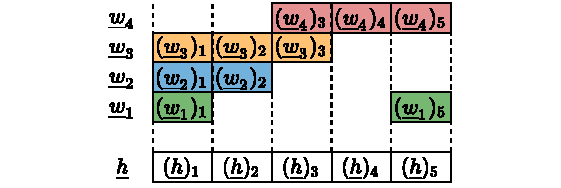
\includegraphics[trim={1.8cm 0 1.7cm 0},clip,scale=0.7]{images/parameter_mapping.pdf}}
    \subfloat[][]{\includestandalone[trim={0.65cm 0 0 0},clip,scale=0.7]{tikz/connection_matrix}}
    \subfloat[][]{\includestandalone[trim={0.6cm 0 0 0},clip,scale=0.6]{tikz/problem_splitting_matrix}}
    % \includestandalone[scale=1]{tikz/topology_general}
    \vspace*{-0.3cm}
    \caption{Problem splitting and parameter mapping for a general case with \(M=5\) channels and \(N=4\) sub-problems. (a) shows the mapping of the local estimate components \((\wf_i)_j\) to the global consensus components \((\hf)_j\) via \(\mathcal{G}(i,j)\), (b) \(\mtxb{G}\) with 1 (\(\blacksquare\)) and 0 (\(\square\)), (c) shows \(i,j\)-cross-relations used by sub-problems compared to full \(M\)-channel problem.}
    \label{fig:problem_splitting:problem_splitting_matrix}
\end{figure}

% #############################################################################
\subsection{General-Form Consensus ADMM}
\label{ssec:general_consensus_admm}
Minimization problems with separable const functions can be solved by the well-established method of consensus ADMM \cite{boydDistributedOptimizationStatistical2011}.
In the previous section we introduced the split cost function \eqref{eq:problem_splitting:cost_function} which we now set in the context of the general-form consensus problem
\begin{align}
    \operatorname{minimize} \quad &\sum_{i \in \Nset} \tilde{J}_i(\wf_i)\\
    \text{subject to} \quad &(\wf_i)_j = \hf_{\mathcal{G}(i,j)},\quad i \in \Nset,\,j \in \Cset_i
\end{align}
where \(\mathcal{G}(i,j)=g\) denotes the mapping of \(L\) local variable components \((\wf_i)_j\), i.e. one of the frequency responses in the stacked vector, to the corresponding global variable components \((\hf)_g\) (cf. \autoref{fig:problem_splitting:problem_splitting_matrix}).
For brevity, the mapped global variables \((\tilde{\hf}_i)_j = \hf_{\mathcal{G}(i,j)}\) are introduced.
The equality constraint between local variables \(\wf_i\) and global variable \(\hf\) enforces the consensus, i.e. a common solution taking into account data of all sub-problems.

The augmented Lagrangian for this particular general-form consensus problem is
% \begin{equation}
%     \mathcal{L}_{\rho} (\wf,\hf,\uuf) = \sum_{i \in \Mset} \left( \wf_i^\herm \aRhof_i \wf_i + 2 \Re \left\{ \uuf_i^{\herm} \left(\wf_i - \tilde{\hf}_i\right) \right\} + \rho \left\| \wf_i - \tilde{\hf}_i \right\|\label{eq:general_consensus_admm:lagrangian}
% \end{equation}
\begin{align}
    &\mathcal{L}_{\rho} (\wf,\hf,\uuf) = \sum_{i \in \Mset} \left( \wf_i^\herm \aRhof_i \wf_i + \uuf_i^{\herm} \left(\wf_i - \tilde{\hf}_i\right)\vphantom{+ \frac{\rho}{2} \left\| \wf_i - \tilde{\hf}_i \right\|^2} \right.\nonumber\\
    &\left. + \left(\wf_i - \tilde{\hf}_i\right)^\herm \uuf_i + \left( \wf_i - \tilde{\hf}_i \right)^\herm \rho \I \left( \wf_i - \tilde{\hf}_i \right) \right).\label{eq:general_consensus_admm:lagrangian}
\end{align}
The ADMM then consists of the steps:
\begin{align}
    \wf_i^{k+1} &= \underset{\wf_i}{\operatorname{argmin}} \, \mathcal{L}_{\rho} (\wf,\hf^k,\uuf^k),\label{eq:general_consensus_admm:local}\\
    \hf^{k+1} &= \underset{\hf, \|\hf\| = a}{\operatorname{argmin}}\, \mathcal{L}_{\rho} (\wf^{k+1},\hf,\uuf^k)\label{eq:general_consensus_admm:global}\\
    \uuf_i^{k+1} &= \uuf_i^{k} + \rho \left( \wf_i^{k+1} - \tilde{\hf}_i^{k+1} \right).\label{eq:general_consensus_admm:dual}
\end{align}
% \begin{align}
%     &\wf_i^{k+1} = \underset{\wf_i}{\operatorname{argmin}} \left\{ \wf_i^\herm \aRhof_i \wf_i + \uuf_i^{k\,\herm} \left(\wf_i - \tilde{\hf}_i^{k}\right) \vphantom{+ \left\| \wf_i - \tilde{\hf}_i^{k} \right\|^2}\right.\nonumber\\
%     &\left.+ \left(\wf_i - \tilde{\hf}_i^{k}\right)^\herm \uuf_i^{k} + \left( \wf_i - \tilde{\hf}_i^{k} \right)^\herm \rho \I \left( \wf_i - \tilde{\hf}_i^{k} \right) \right\},\label{eq:general_consensus_admm:local}\\
%     &\hf^{k+1} = \underset{\hf, \|\hf\| = a}{\operatorname{argmin}} \left\{ \sum_{i \in \Mset} \left( \tilde{\hf}_i^{\herm} \uuf_i^{k} + \uuf_i^{k\,\herm} \tilde{\hf}_i \vphantom{\frac{\rho}{2} \| \wf_i^{k+1} - \tilde{\hf}_i \|^2} \right.\right.\nonumber\\
%     &\left. \qquad \qquad \vphantom{\sum_{i=1}^{M} pp } \left.+ \left( \wf_i^{k+1} - \tilde{\hf}_i \right)^\herm \rho \I \left( \wf_i^{k+1} - \tilde{\hf}_i \right)  \right) \right\},\label{eq:general_consensus_admm:global}\\
%     &\uuf_i^{k+1} = \uuf_i^{k} + \rho \left( \wf_i^{k+1} - \tilde{\hf}_i^{k+1} \right).\label{eq:general_consensus_admm:dual}
% \end{align}
As this is still denoted as an iterative method, we will introduce the online/adaptive aspect of the proposed method next.

\subsection{Online ADMM-BSI}
\label{ssec:online_admm}
We introduced the original problem \eqref{eq:frequency_domain:null_space} with time-dependent data matrix. Following from this, also the data term in \eqref{eq:general_consensus_admm:lagrangian} is time-dependent, which from here on out will be denoted with the additional superscript time index \(m\) as \(\wf_i^\herm \aRhof_i^{m} \wf_i\).
A thorough look at time-varying data terms in ADMM can be found in \cite{wangOnlineAlternatingDirection2013,hosseiniOnlineDistributedADMM2014} where it is referred to as "Online-ADMM".

We transform the iterative batch processing method \eqref{eq:general_consensus_admm:local}-\eqref{eq:general_consensus_admm:dual} into an adaptive one by computing only a (small) finite number of iterations with each time-frame-\(m\) specific data term.
Here specifically, we apply one iteration per time frame, which manifests itself as simply replacing the iteration index \(k\) with the time index \(m\)

The minimization problem for the local variable \(\wf_i\) \eqref{eq:general_consensus_admm:local} can be solved by various methods, in this case however we perform a Newton update step
\begin{equation}
    \wf_i^{m+1} = \wf_i^{m} - \mu \bm{{V}}_i^m \left( \aRhof_i^m \wf_i^m + \uuf_i^m + \rho\left(\wf_i^m - \tilde{\hf}_i^{m}\right)\right)\label{eq:online_admm:local_update}
\end{equation}
where \(0  < \mu\leq 1\) is a step size and \(\bm{{V}}_i^m = \left(\aRhof_i^m + \rho \I \right)^{-1}\) is the inverse Hessian of the problem.
As this inverse is costly to compute, it is approximated by a diagonalized matrix
\begin{equation}
    \tilde{\bm{{V}}}_i^m = \operatorname{diag} \left\{ \left( \operatorname{diag} \left\{ \aRhof_i^m \right\} + \rho \mtxb{1} \right)^{-1}\right\},
\end{equation}
similar to NMCFLMS \cite{huangClassFrequencydomainAdaptive2003}, which is straightforward to compute.

For the update step of the consensus variable \(\hf\), it may be readily verified (cf. \cite{boydDistributedOptimizationStatistical2011}) that the solution to \eqref{eq:general_consensus_admm:global} is given by
\begin{equation}
    \hf^{m+1} = a\frac{\bar{\wf}^{m+1} + \frac{1}{\rho} \bar{\uuf}^{m} }{\left\| \bar{\wf}^{m+1} + \frac{1}{\rho} \bar{\uuf}^{m} \right\|}.\label{eq:online_admm:consensus_update}
\end{equation}
where the \(M L \times 1\) vectors \(\bar{\wf}^{m+1}, \bar{\uuf}^{m+1}\) are computed as the mapped averages
\begin{equation}
    (\bar{\wf}^{m+1})_g = \frac{1}{N_g} \sum_{\mathcal{G}(i,j)=g} (\wf_i^{m+1})_j,\quad g,i,j \in \Mset,
\end{equation}
and
\begin{equation}
    (\bar{\uuf}^{m})_g = \frac{1}{N_g} \sum_{\mathcal{G}(i,j)=g} (\uuf_i^{m})_j,\quad g,i,j \in \Mset.
\end{equation}
This results in a computationally inexpensive update step forcing the norm of the consensus to have value \(a\).

% #############################################################################
% #############################################################################
\section{Numerical Evaluation}
\label{sec:perf_eval}

\begin{figure}[t]
    \centering
    \subfloat[][]{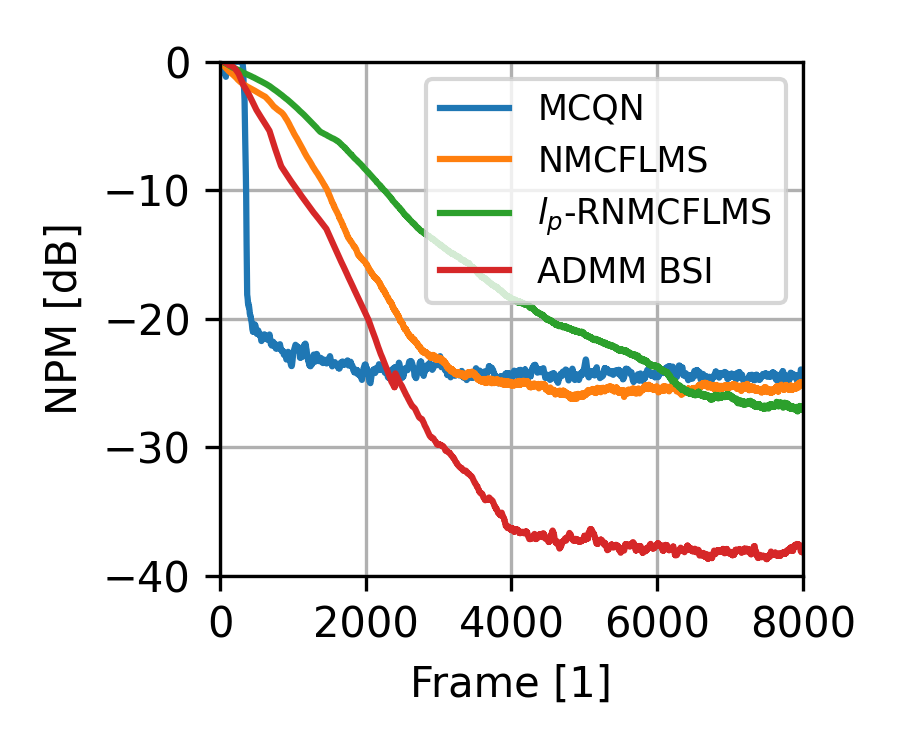
\includegraphics[trim={0.3cm 0.35cm 0.3cm 0.3cm},clip,height=4cm]{python/plots/NPM_over_time_SNR10.png}\label{fig:perf_eval:NPM_over_time_SNR10}}\\
    \vspace*{-0.3cm}
    \subfloat[][]{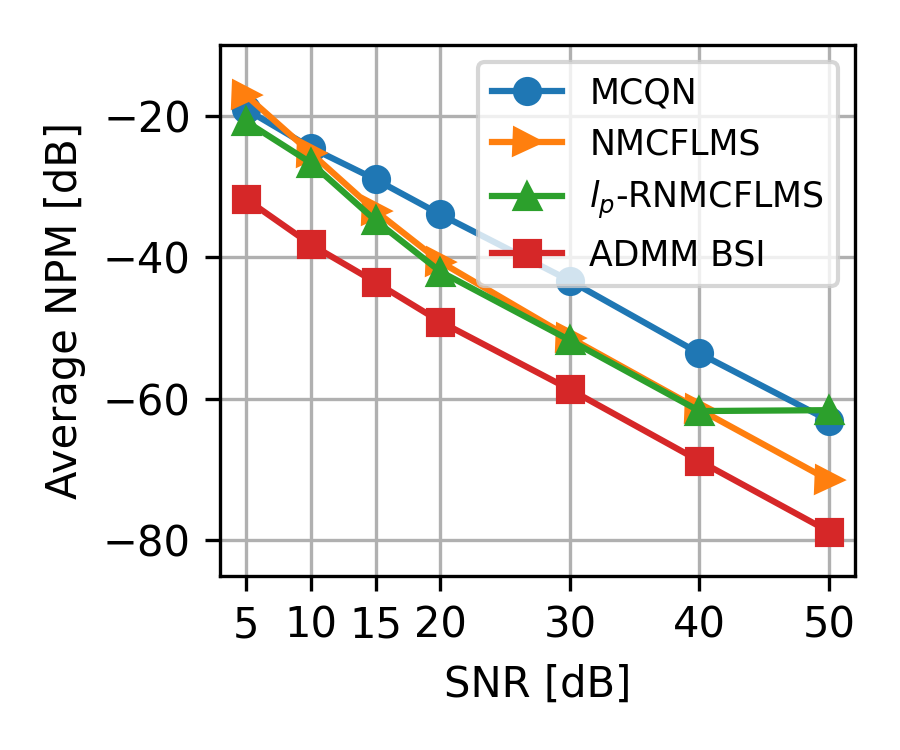
\includegraphics[trim={0.3cm 0.35cm 0.3cm 0.3cm},clip,height=4cm]{python/plots/NPM_over_SNR_L64_M5.png}\label{fig:perf_eval:NPM_over_SNR_L64_M5}}
    \vspace*{-0.2cm}
    \caption{Comparison of ADMM-BSI convergence behaviour with \(L\!=\!64\) at different SNR values. Shown are (a) NPM at \(\text{SNR}=10\,\text{dB}\) over frame index \(m\) for convergence speed comparison and (b) the steady-state NPMs over different SNRs.}
    \label{fig:perf_eval:NPM_over_time_exp1}
\end{figure}

The performance of the proposed algorithm is assessed via numerical simulations.
As error measure, we use the normalized projection misalignment (NPM) \cite{huangClassFrequencydomainAdaptive2003}
\begin{equation}
    \text{NPM}(m) = 20\,\log_{10} \left(\frac{\left\| \h(m) - \frac{\h^\T (m) \h_{\text{t}}}{\h_{\text{t}}^\T \h_{\text{t}}}\h(m) \right\|_2}{\left\|\h(m)\right\|_2} \right)
\end{equation}
where \(\h\) is the stacked vector of impulse response estimates (cf. \autoref{ssec:cross_rel}), which are the inversely Fourier-transformed estimated frequency responses stacked in \(\hf\) and \(\h_{\text{t}}\) is the ground truth.

Further, the signal-to-noise ratio (SNR) for the experiments is defined as 
\begin{equation}
    \text{SNR} = 10 \log_{10} \left(\frac{\sigma_s^2 \| \h_t \|}{M \sigma_v^2} \right)
\end{equation}
where \(\sigma_s^2\) and \(\sigma_v^2\) are the variance of signal and noise respectively which both are modelled by (channel-independent) white Gaussian noise (WGN).

The first experiment evaluates the performance using randomly generated impulse responses of length \(L=64\) under different signal-to-noise ratios (SNR) on a 5-channel system (\(M=5,\,N=5\)).
The impulse responses are drawn from a Normal distribution with unit variance, and the signal is 100 seconds (\(f_s=8000\)) of WGN to ensure convergence of all algorithms.
The step sizes are hand tuned for stable convergence: \(\mu_{\text{MCQN}}=0.5,\, \mu_{\text{NMCFLMS}}=0.4,\, \mu_{l_p-\text{NMCFLMS}}=0.3,\, \mu_{\text{ADMM}}=0.6,\, \rho=1,\,\eta=0.98 \).
\autoref{fig:perf_eval:NPM_over_time_exp1} shows the median of 30 Monte-Carlo runs where the averaged NPM of the last \(100\) frames is taken as measurement.
It is observable that the proposed algorithm yields a lower steady-state NPM than the compared NMCFLMS, RNMCFLMS, and \(l_p\)-RNMCFLMS algorithms.

\begin{figure}[t]
    \centering
    % \hspace*{-0.4cm}\subfloat[][\(M\!=\!4,P\!=\!4\)]{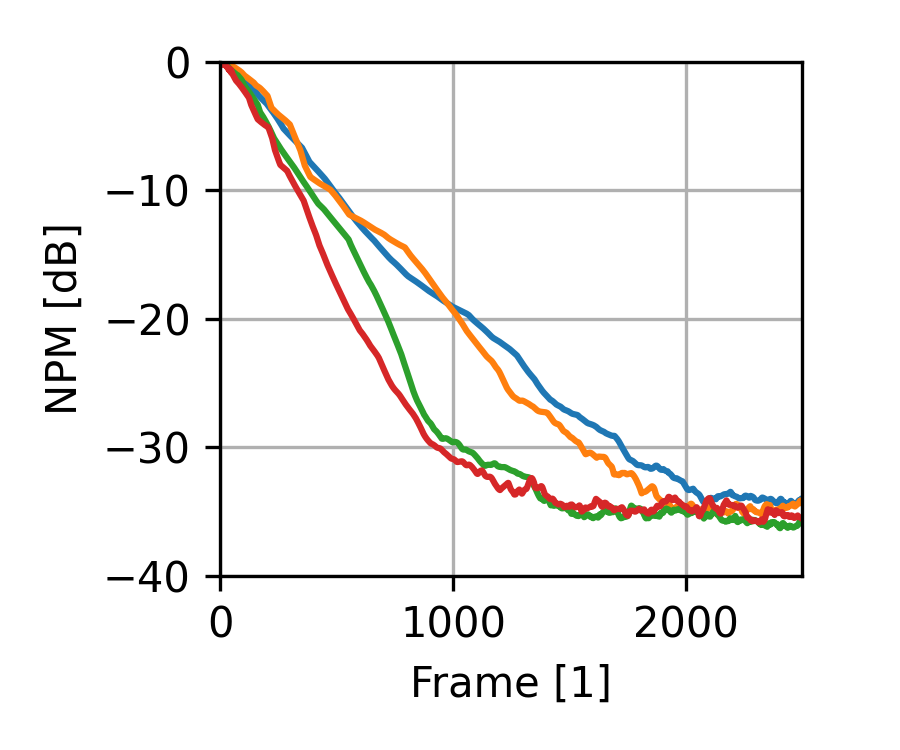
\includegraphics[height=4cm]{python/plots/NPM_over_time_M4.png}\label{fig:perf_eval:NPM_over_time_M4}}
    \hspace*{-0.2cm}\subfloat[][\(M\!=\!4,N\!=\!4\)]{\begin{overpic}[trim={0.3cm 0.35cm 0.3cm 0.3cm},clip,height=3.7cm]{python/plots/NPM_over_time_M4.png}
        \put(54,48){\includestandalone[trim={0.0cm 0.0cm 0.0cm 0},clip,scale=0.5]{tikz/connection_matrix_eval}}
    \end{overpic}\label{fig:perf_eval:NPM_over_time_M4}}
    \hspace*{-0.0cm}\subfloat[][\(M\!=\!8,N\!=\!8\)]{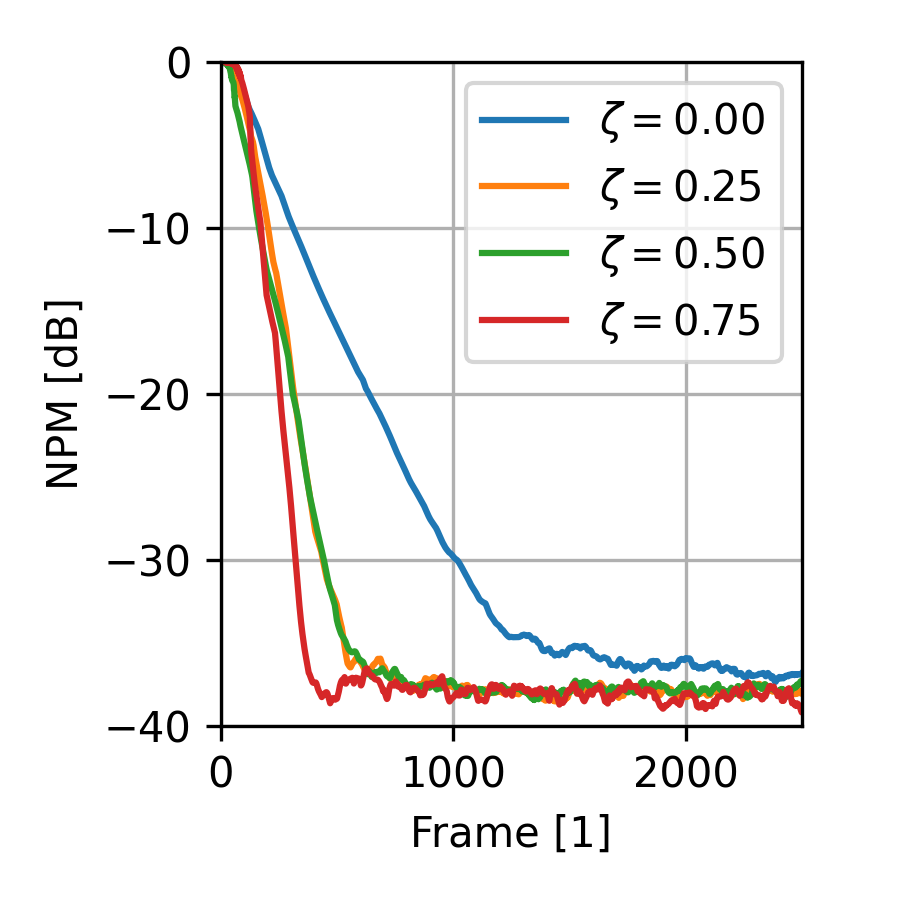
\includegraphics[trim={0.3cm 0.35cm 0.3cm 0.3cm},clip,height=3.7cm]{python/plots/NPM_over_time_M8.png}\label{fig:perf_eval:NPM_over_time_M8}}
    \vspace*{-0.2cm}
    \caption{Comparison of ADMM-BSI convergence behaviour with \(L\!=\!16\) for different values of the sub-problem overlap \(\zeta\).}
    \label{fig:perf_eval:NPM_over_time_exp2}
\end{figure}

The second experiment is a small-scale assessment of the influence of the overlap of sub-problems.
Two base scenarios, \(M=4,\,N=4\) and \(M=8,\,N=8\), are evaluated using short (\(L=16\)) random impulse responses and different values for the sub-problem overlap parameter \(\zeta\) which is defined as the ratio of ones to zeros of only considering elements of \(\mtxb{G}\) that are not part of the main diagonal, superdiagonal and the first element of the last row (marked gray in \autoref{fig:perf_eval:NPM_over_time_M4}).
Random patterns satisfying this definition for \(\zeta \in \{0.0,\,0.25,\,0.5,\,0.75\}\) are generated.
\autoref{fig:perf_eval:NPM_over_time_exp2} shows the median of 30 Monte-Carlo runs for the two setups, which shows the proportional relation of convergence speed, channel number \(M\) and sub-problem overlap \(\zeta\).
Note that the steady-state error is not dependent on \(\zeta\).




% #############################################################################
% #############################################################################
\section{Conclusions}
\label{sec:conclusion}
In this paper, a novel adaptive ADMM algorithm for blind system identification was developed.
The algorithm separates the BSI problem into lower-dimensional sub-problems to reduce complexity and allow parallel processing while maintaining steady-state error performance and convergence speed.
Comparison to state-of-the-art algorithms in numerical simulations shows improved steady-state error measures for randomly generated impulse responses.
A further experiment to assess the influence of sub-problem overlap shows that steady-state performance is not affected by the separation while convergence speed is.

% References should be produced using the bibtex program from suitable
% BiBTeX files (here: strings, refs, manuals). The IEEEbib.bst bibliography
% style file from IEEE produces unsorted bibliography list.
% -------------------------------------------------------------------------
\bibliographystyle{IEEEbib}
\bibliography{iwaenc2022}

\end{document}